\def\duedate{September 5, 2023}
\def\HWnum{1}
\documentclass[10pt,a4paper]{book}

% custom section formatting
\usepackage{titlesec}
\titleformat{\chapter}[display]
{\normalfont\Large\filcenter\sffamily}
{\titlerule[1pt]%
\vspace{1pt}%
\titlerule
\vspace{1pc}%
\LARGE\MakeUppercase{\chaptertitlename} \thechapter}
{1pc}
{\titlerule
\vspace{1pc}%
\Huge}

% appendix handling
\usepackage[toc,page]{appendix}
    
% encoding for file and font
\usepackage[utf8]{inputenc}
\usepackage[T1]{fontenc}

% math formatting/tools
\usepackage{amsmath}
\usepackage{amssymb}
\usepackage{mathtools}
\usepackage[arrowdel]{physics}

% unit formatting
\usepackage{siunitx}
\AtBeginDocument{\RenewCommandCopy\qty\SI}

% figure formatting/tools
\usepackage{graphicx}
\usepackage{float}
\usepackage{subcaption}
\usepackage{multirow}
\usepackage{import}
\usepackage{pdfpages}
\usepackage{transparent}
\usepackage{currfile}

\NewDocumentCommand\incfig{O{1} m}{
    \def\svgwidth{#1\textwidth}
    \import{./Figures/\currfiledir}{#2.pdf_tex}
}

\newcommand{\bef}{\begin{figure}[h!tb]\centering}
\newcommand{\eef}{\end{figure}}

\newcommand{\bet}{\begin{table}[h!tb]\centering}
\newcommand{\eet}{\end{table}}

% hyperlink references 
\usepackage{hyperref}
\hypersetup{
    colorlinks=true,
    linkcolor=blue,
    filecolor=magenta,
    urlcolor=cyan,
    pdftitle={Physics 1 Notes},
    pdfauthor={Richard Whitehill},
    pdfpagemode=FullScreen
}
\urlstyle{same}

\newcommand{\eref}[1]{Eq.~(\ref{eq:#1})}
\newcommand{\erefs}[2]{Eqs.~(\ref{eq:#1})--(\ref{eq:#2})}

\newcommand{\fref}[1]{Fig.~(\ref{fig:#1})}
\newcommand{\frefs}[2]{Fig.~(\ref{fig:#1})--(\ref{fig:#2})}

\newcommand{\aref}[1]{Appendix~(\ref{app:#1})}
\newcommand{\sref}[1]{Section~(\ref{sec:#1})}
\newcommand{\srefs}[2]{Sections~(\ref{sec:#1})-(\ref{sec:#2})}

\newcommand{\tref}[1]{Table~(\ref{tab:#1})}
\newcommand{\trefs}[2]{Table~(\ref{tab:#1})--(\ref{tab:#2})}

% tcolorbox formatting/definitions
\usepackage[most]{tcolorbox}
\usepackage{xcolor}
\usepackage{xifthen}
\usepackage{parskip}

\definecolor{peach}{rgb}{1.0,0.8,0.64}

\DeclareTColorBox[auto counter, number within=chapter]{defbox}{O{}}{
    enhanced,
    boxrule=0pt,
    frame hidden,
    borderline west={4pt}{0pt}{green!50!black},
    colback=green!5,
    before upper=\textbf{Definition \thetcbcounter \ifthenelse{\isempty{#1}}{}{: #1} \\ },
    sharp corners
}

\newcommand*{\eqbox}{\tcboxmath[
    enhanced,
    colback=black!10!white,
    colframe=black,
    sharp corners,
    size=fbox,
    boxsep=8pt,
    boxrule=1pt
]}

\newtcolorbox[auto counter, number within=chapter]{exbox}{
    parbox=false,
    breakable,
    enhanced,
    sharp corners,
    boxrule=1pt,
    colback=white,
    colframe=black,
    before upper= \textbf{Example \thetcbcounter:}\,,
    before lower= \textbf{Solution:}\,,
    segmentation hidden
}

\newtcolorbox{resbox}{
    enhanced,
    colback=black!10!white,
    colframe=black,
    boxrule=1pt,
    boxsep=0pt,
    top=2pt,
    ams nodisplayskip,
    sharp corners
}


\begin{document}

\prob{1}{
Calculate the curls of vector functions
\begin{enumerate}[label=\alph*)]
    \item $\va*{v}_{a} = x^2 \vu*{e}_{1} + 3xz^2 \vu*{e}_{2} - 2xz \vu*{e}_{3}$
    \item $\va*{v}_{b} = xy \vu*{e}_{1} + 2yz \vu*{e}_{2} + 3xz \vu*{e}_{3}$
\end{enumerate}
}

\sol{

    a) The curl of a vector $\va*{v}$ is $\displaystyle \curl{\va*{v}} = \Big( \pdv{v_{z}}{y} - \pdv{v_{y}}{z} \Big) \vu*{e}_{1} + \Big( \pdv{v_{x}}{z} - \pdv{v_{z}}{x} \Big) \vu*{e}_{2} + \Big( \pdv{v_{y}}{x} - \pdv{v_{x}}{y} \Big) \vu*{e}_{1}$.
    Hence,
    \begin{eqnarray}
        \curl{\va*{v}_{a}} = -6xz \vu*{e}_{1} + 2z \vu*{e}_{2} + 3z^2 \vu*{e}_{3}
    .\end{eqnarray}
    
b) The curl of $\va*{v}_{b}$ is 
\begin{eqnarray}
   \curl{\va*{v}_{b}} = -2y \vu*{e}_{1} - 3z \vu*{e}_{2} - x \vu*{e}_{3}
.\end{eqnarray}

}

\prob{2}{
Check the fundamental theorem for gradients
\begin{eqnarray}
    \label{eq:ftg}
    \int_{\va*{a}~{\cal P}}^{\va*{b}} \grad{T} \cdot \dd{\va*{l}} = T(\va*{b}) - T(\va*{a})
\end{eqnarray}
using $T = x^2 + 4xy + 2yz^3$, the points $\va*{a} = (0,0,0)$, $\va*{b} = (1,1,1)$ and the two paths $\mathcal{P}$ shown below:
\begin{enumerate}[label=\alph*)]
    \item $(0,0,0) \rightarrow (0,0,1) \rightarrow (0,1,1) \rightarrow (1,1,1)$
    \item the parabolic path $x = y$, $z = x^2$
\end{enumerate}
}

\begin{figure}[!htb]
    \centering
    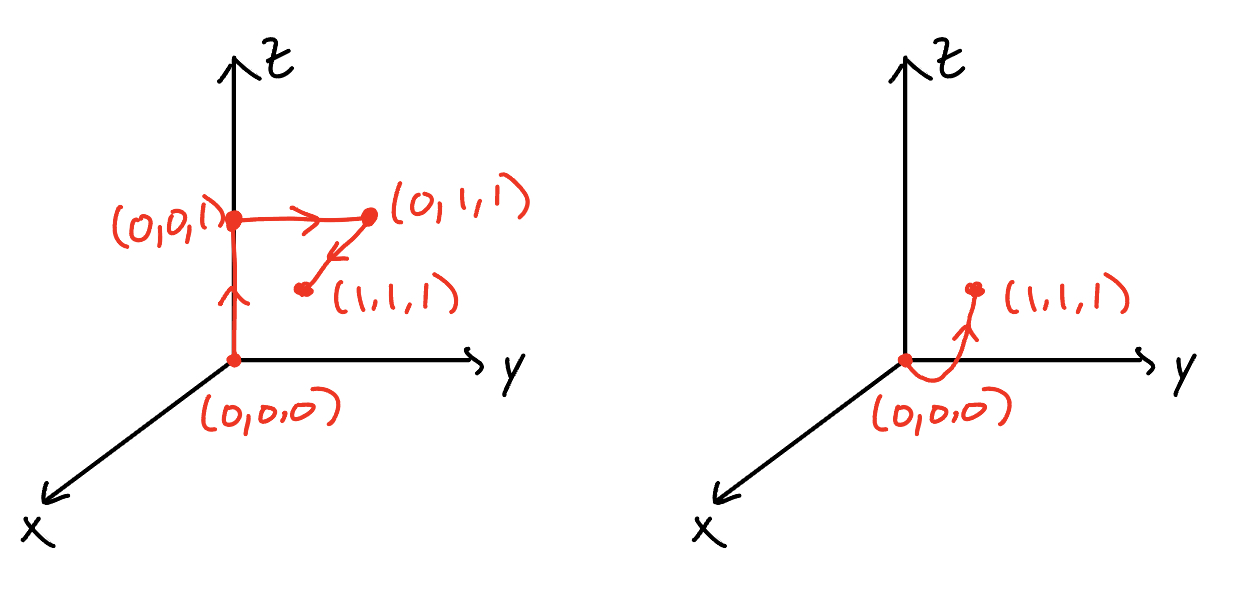
\includegraphics[width=0.5\textwidth]{prob2.jpeg}
    \label{fig:prob2}
    \caption{\textbf{Left} -- path taken in part (a) and \textbf{Right} -- path taken in part (b).}
\end{figure}

\sol{

    The right hand side of the equation is simply $T(1,1,1) - T(0,0,0) = 7$.

    The gradient of $T$ is given as $\grad{T} = \partial_{x} T \, \vu*{x} + \partial_{y} T \, \vu*{y} + \partial_{z} T \, \vu*{z} = \\ (2x + 4y) \vu*{x} + (4x + 2z^3) \vu*{y} + 6yz^2 \vu*{z}$

    a) This path integral can be broken over the individual line segments as\footnote{excuse the abuse of notation}
\begin{eqnarray}
    \int_{\cal P} = \int_{(0,0,0)}^{(0,0,1)} + \int_{(0,0,1)}^{(0,1,1)} + \int_{(0,1,1)}^{(1,1,1)}
.\end{eqnarray}

Generally for a line passing through $\va*{a}$ and $\va*{b}$, we can write the equation of such a line in terms of the independent parameter $t$ as $\va*{r} = \va*{a} + (\va*{b} - \va*{a})t$.
Hence the generic path integral over a line from $\va*{a}$ to $\va*{b}$ may be written as
\begin{eqnarray}
    \int_{\va*{a}}^{\va*{b}} \va*{F} \cdot \dd{\va*{l}} = \int_{0}^{1} \va*{F} \cdot \dv{\va*{l}}{t} \dd{t}
.\end{eqnarray}

The line integral over the path specified is then
\begin{eqnarray}
    \begin{aligned}    
        \int_{\cal P} \grad{T} \cdot \dd{\va*{l}} &= \int_{0}^{1} \grad{T} \cdot \vu*{z} \dd{t} + \int_{0}^{1} \grad{T} \cdot \vu*{y} \dd{t} + \int_{0}^{1} \grad{T} \cdot \vu*{x} \dd{t} \\
                                                  &= 0 + \int_{0}^{1} 2 \dd{t} + \int_{0}^{1} (2t + 4) \dd{t} = \eqbox{7}
    \end{aligned}
\end{eqnarray}
as expected.

b) In this problem, we can use $x$ as our independent parameter and write $\va*{l} = x \vu*{x} + x \vu*{y} + x^2 \vu*{z}$, which gives $\dv{\va*{l}}{x} = \vu*{x} + \vu*{y} + 2x \vu*{z}$.
The path integral is then
\begin{eqnarray}
    \int_{\cal P} \grad{T} \cdot \dd{\va*{l}} = \int_{0}^{1} [ 6x + (4x + 2x^{6}) + 2x(6x^5) ] \dd{x} = \int_{0}^{1} (14x^{6} + 10x) \dd{x} = \eqbox{7}
.\end{eqnarray}


}

\prob{3}{
Check Stoke's theorem
\begin{eqnarray}
    \int (\curl{\va*{v}}) \cdot \dd{\va*{a}} = \oint_{\mathcal{P}} \va*{v} \cdot \dd{\va*{l}}
.\end{eqnarray}
for the function $\va*{v} = xy \vu*{e}_{1} + 2yz \vu*{e}_{2} + 3xz \vu*{e}_{3}$ using the triangular shaded area shown below.
}

\begin{figure}[!htb]
   \centering
   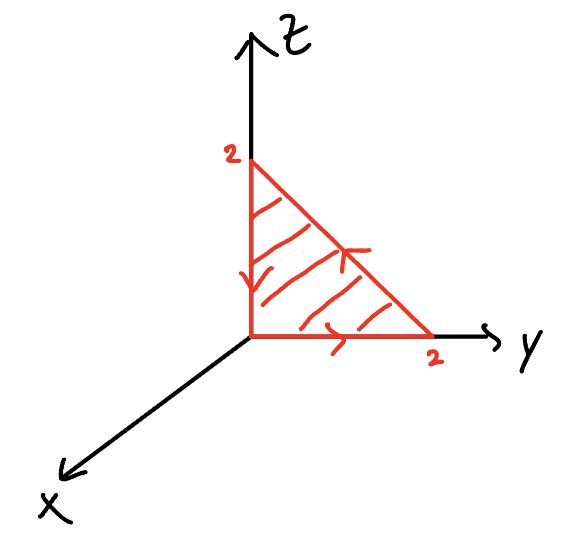
\includegraphics[width=0.4\textwidth]{prob3.jpeg}
   \label{fig:prob3}
   \caption{The triangular region to perform integration over. Note that in the original figure there is no orientation specified for the path integral, and therefore is a bit vague since there are two unit normal vectors to the surface shown (in the sense that there are two directions for the normal vector to point). In either case, the equality holds, but for concreteness, we choose the path to be oriented counter-clockwise and the normal vector to therefore be $\vu*{x}$.}
\end{figure}

\sol{

We do the left hand side first.
The curl of the $\va*{v}$ is $\curl{\va*{v}} = -2y \vu*{x} - 3z \vu*{y} - x \vu*{z}$, and the surface integral is
\begin{eqnarray}
\int (\curl{\va*{v}}) \cdot \vu*{x} \dd{y} \dd{z} = \int_{0}^{2} \int_{0}^{2-z} -2y \dd{y} \dd{z} = - \int_{0}^{2} (2-z)^2 \dd{z} = \eqbox{ -\frac{8}{3} }
.\end{eqnarray}

Now for the right side.
The integral can be written
\begin{eqnarray}
\begin{aligned}
    \oint_{\cal P} \va*{v} \cdot \dd{\va*{l}} &= \int_{\va*{0}}^{2\vu*{y}} \va*{v} \cdot \dd{\va*{l}} + \int_{2\va*{y}}^{2\vu*{z}} \va*{v} \cdot \dd{\va*{l}} + \int_{2\vu*{z}}^{\va*{0}} \va*{v} \cdot \dd{\va*{l}} \\
                                              &= \int_{0}^{1} \va*{v} \cdot 2 \vu*{y} \dd{t} + \int_{0}^{1} \va*{v} \cdot 2(\vu*{z} - \vu*{y}) \dd{t} + \int_{0}^{1} \va*{v} \cdot (-2 \vu*{z}) \dd{t} \\
                                              &= 2 \Bigg[ 0 - \int_{0}^{1} 2(2-t)t \dd{t} + 0 \Bigg] = \eqbox{ -\frac{8}{3} }
.\end{aligned}
\end{eqnarray}


}

\end{document}
